% =============================================================================
% math-function-plot.tex — Cartesian axes with a plotted curve and annotations
%
% Shows: f(x) = x^2 - 2 on labelled axes, with its two roots marked, the
% vertex marked, and the curve labelled at its right end.
% Compiles standalone via: xelatex math-function-plot.tex
%
% Use for: calculus, precalculus, numerical methods (root finding), any
% "here is the function we are about to analyse" slide.
%
% AXES EXTEND BEYOND THE DATA on every side — see tikz-visual-quality.md. If
% you change the function, re-check that the axis ranges still bracket it.
% =============================================================================

\documentclass[border=5pt]{standalone}
\usepackage{tikz}
\usetikzlibrary{arrows.meta, positioning}

\definecolor{axis}{HTML}{1A1A1A}
\definecolor{curve}{HTML}{012169}
\definecolor{root}{HTML}{B91C1C}
\definecolor{vertex}{HTML}{15803D}
\definecolor{muted}{HTML}{525252}

\tikzset{
  axisline/.style={-{Latex[length=2.6mm]}, thick, draw=axis},
  curveline/.style={thick, draw=curve, smooth},
  gridline/.style={draw=muted!35, very thin},
  ticklbl/.style={font=\scriptsize, text=muted},
  ptdot/.style={circle, fill=root, minimum size=4pt, inner sep=0pt},
  vdot/.style={circle, fill=vertex, minimum size=4pt, inner sep=0pt}
}

% -----------------------------------------------------------------------------
% Diagram: f(x) = x^2 - 2 on x in [-2.4, 2.4].
% Scale: 1 unit x = 1.5cm, 1 unit y = 0.9cm (set via the plot expression, NOT
% via `scale=`, which tikz-prevention.md P3 bans because it shrinks coordinates
% without shrinking text).
% Data range: f(-2.4) = 3.76 (top), f(0) = -2 (bottom).
% Axes therefore run x in [-2.9, 2.9]*1.5 and y in [-2.6, 4.3]*0.9, i.e. they
% extend past the data on all four sides.
% Roots at x = +/- sqrt(2) ~= +/- 1.414 -> plotted at x = +/- 2.121cm.
% Labels sit ABOVE-RIGHT of their dots so they never sit on the curve (P7b).
% -----------------------------------------------------------------------------

\begin{document}
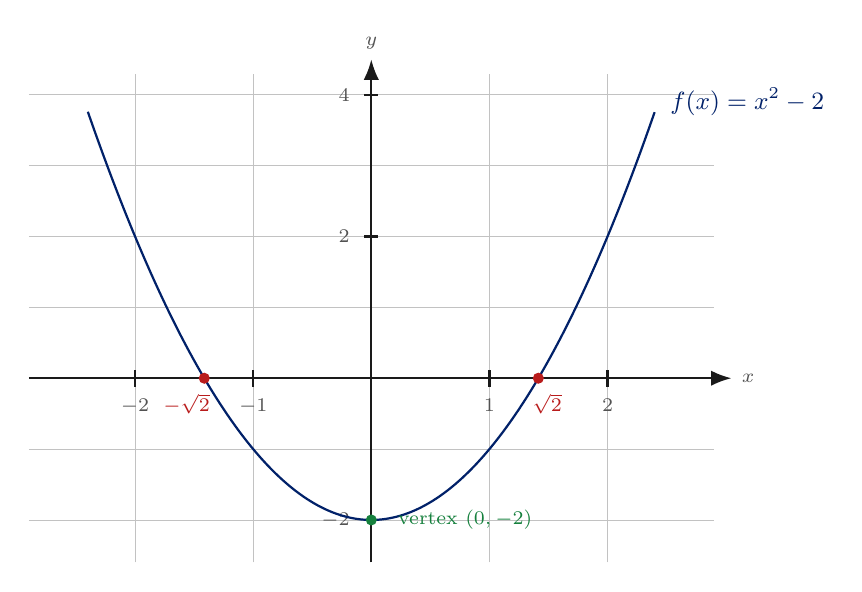
\begin{tikzpicture}[
    x=1.5cm, y=0.9cm,
    declare function={f(\x) = \x*\x - 2;}
  ]

  % ---- Light grid ----------------------------------------------------------
  \foreach \gx in {-2,-1,1,2} { \draw[gridline] (\gx, -2.6) -- (\gx, 4.3); }
  \foreach \gy in {-2,-1,1,2,3,4} { \draw[gridline] (-2.9, \gy) -- (2.9, \gy); }

  % ---- Axes ----------------------------------------------------------------
  \draw[axisline] (-2.9, 0) -- (3.05, 0) node[right, ticklbl] {$x$};
  \draw[axisline] (0, -2.6) -- (0, 4.5)  node[above, ticklbl] {$y$};

  % ---- Ticks ---------------------------------------------------------------
  \foreach \tx in {-2,-1,1,2} {
    \draw[thick, draw=axis] (\tx, -0.12) -- (\tx, 0.12);
    \node[ticklbl, below] at (\tx, -0.16) {$\tx$};
  }
  \foreach \ty in {-2,2,4} {
    \draw[thick, draw=axis] (-0.06, \ty) -- (0.06, \ty);
    \node[ticklbl, left] at (-0.10, \ty) {$\ty$};
  }

  % ---- The curve -----------------------------------------------------------
  \draw[curveline, domain=-2.4:2.4, samples=80]
        plot (\x, {f(\x)});

  % ---- Curve label, at the right end, offset above the curve --------------
  \node[text=curve, font=\small, right] at (2.45, 3.90) {$f(x) = x^2 - 2$};

  % ---- Roots ---------------------------------------------------------------
  \node[ptdot] (r1) at (-1.4142, 0) {};
  \node[ptdot] (r2) at ( 1.4142, 0) {};
  \node[font=\scriptsize, text=root, below left=0.02cm and -0.25cm of r1]
        {$-\sqrt{2}$};
  \node[font=\scriptsize, text=root, below right=0.02cm and -0.25cm of r2]
        {$\sqrt{2}$};

  % ---- Vertex --------------------------------------------------------------
  \node[vdot] (v) at (0, -2) {};
  \node[font=\scriptsize, text=vertex, right=0.14cm of v] {vertex $(0,-2)$};

\end{tikzpicture}
\end{document}
